%!TEX root = ../Thesis.tex
\chapter{Background}

% \begin{figure}[h]
%     \centering
%         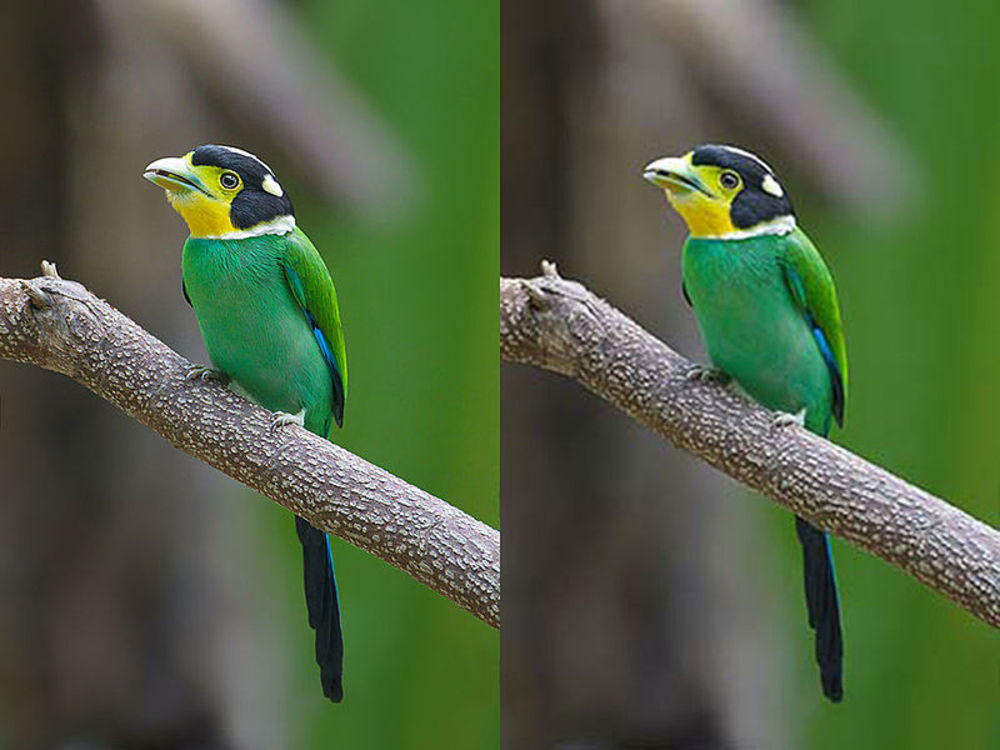
\includegraphics[width=0.8\textwidth]{../graphics/jpeg_compression_example.jpg}
%     \caption[Short caption to special figure]{\textit{Left:} Original image . \textit{Right:} The same image after JPEG compression. Note the blocking artifacts in the background, and the ringing artifacts near edges. \tiny{By Ibrahim.ID (Psarisomus dalhousiae - Kaeng Krachan.jpg) [CC-BY-SA-3.0 (http://creativecommons.org/licenses/by-sa/3.0)], via Wikimedia Commons}}
%     \label{compressionExample}
% \end{figure}

\section{JPEG compression}


\emph{JPEG} is a lossy compression method for digital images. It was named after the \emph{Joint Photographics Experts Group} which authored the standard. This method aims to make the image more compressible by throwing away information which leads to a small difference in perceived quality. In particular it removes high frequency changes in intensity, and often also hue information but not brightness.

\begin{figure}[ht]
\centering
\begin{subfigure}{.33\textwidth}
  \centering
  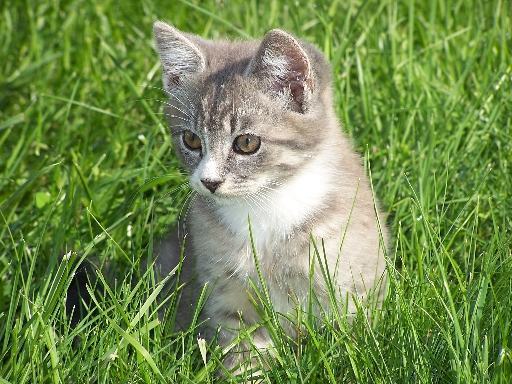
\includegraphics[width=.98\linewidth]{../images/compression_examples/original}
  \caption{Original image}
\end{subfigure}%
\begin{subfigure}{.33\textwidth}
  \centering
  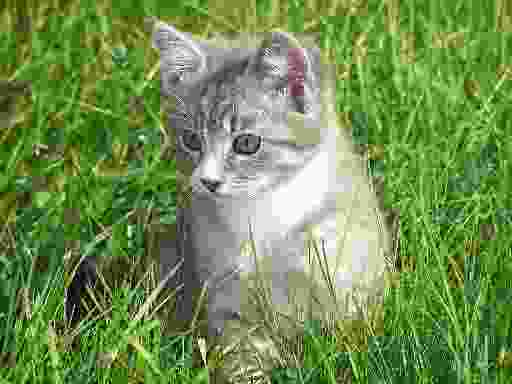
\includegraphics[width=.98\linewidth]{../images/compression_examples/qf5}
  \caption{$QF=5$}
\end{subfigure}%
\begin{subfigure}{.33\textwidth}
  \centering
  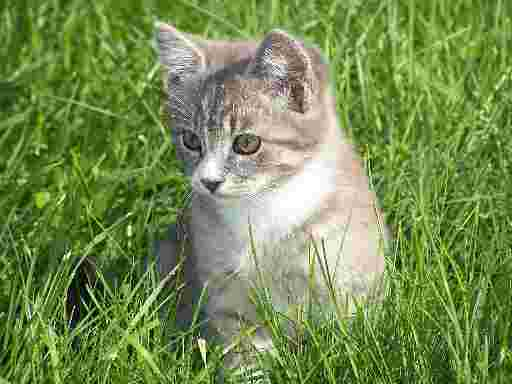
\includegraphics[width=.98\linewidth]{../images/compression_examples/qf10}
  \caption{$QF=10$}
\end{subfigure}
\begin{subfigure}{.33\textwidth}
  \centering
  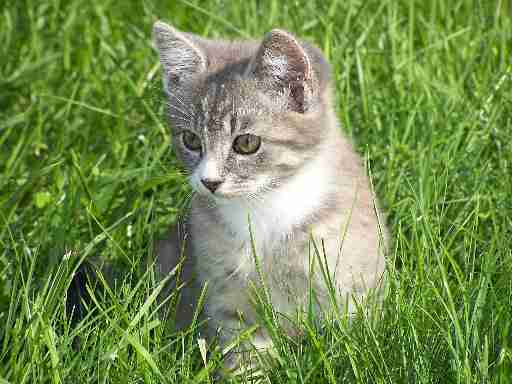
\includegraphics[width=.98\linewidth]{../images/compression_examples/qf20}
  \caption{$QF=20$}
\end{subfigure}%
\begin{subfigure}{.33\textwidth}
  \centering
  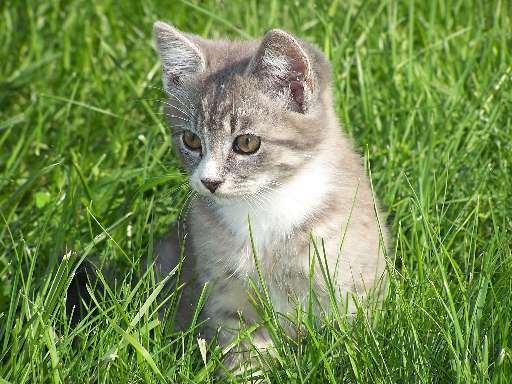
\includegraphics[width=.98\linewidth]{../images/compression_examples/qf60}
  \caption{$QF=50$}
\end{subfigure}%
\begin{subfigure}{.33\textwidth}
  \centering
  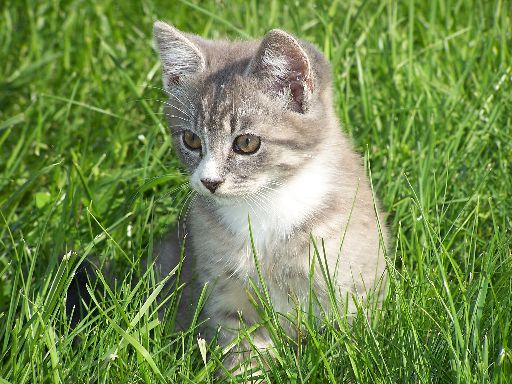
\includegraphics[width=.98\linewidth]{../images/compression_examples/qf80}
  \caption{$QF=80$}
\end{subfigure}%
\caption{Example image after JPEG compression with varying quality factors. Blocking artifacts and hue information loss are especially visible with low quality factor settings.}
\label{fig_compression_qf}
\end{figure}%


JPEG compression has one main parameter, the \emph{quality factor (QF)}, which is a value between 0 and 100. A lower quality factor means that more high frequency information is thrown away, which allows for a greater compression ratio, but at the cost of quality loss. In figure \ref{fig_compression_qf} an image is shown at various quality factor settings.


\subsection{JPEG compression overview}

Different encoding methods exist within the JPEG standard, but the most common is JFIF encoding which consists roughly of the following steps:


\begin{figure}[ht]
\centering
\begin{subfigure}{.33\textwidth}
  \centering
  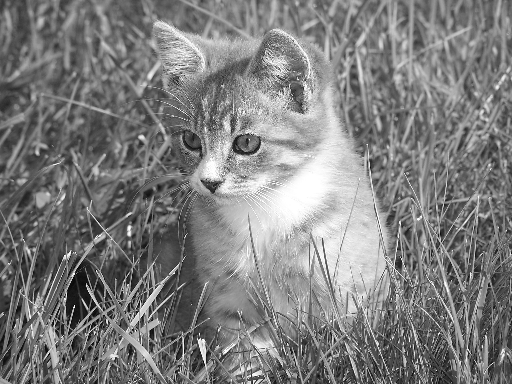
\includegraphics[width=.98\linewidth]{../images/compression_examples/ycrcb_0}
  \caption{Luma ($Y$) }
\end{subfigure}%
\begin{subfigure}{.33\textwidth}
  \centering
  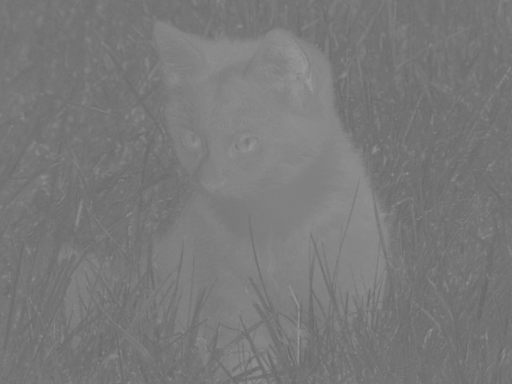
\includegraphics[width=.98\linewidth]{../images/compression_examples/ycrcb_1}
  \caption{Blue difference ($C_b$)}
\end{subfigure}%
\begin{subfigure}{.33\textwidth}
  \centering
  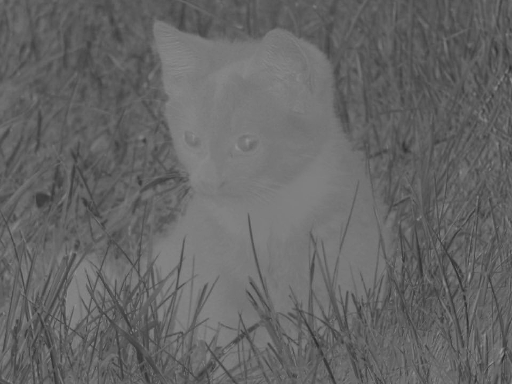
\includegraphics[width=.98\linewidth]{../images/compression_examples/ycrcb_2}
  \caption{Red difference ($C_r$)}
\end{subfigure}%
\caption{Color components of our example image in $Y'C_BC_R$ color space.}
\label{fig_compression_qf}
\end{figure}
%\todo{Show Cb and Cr components in their RGB representation.}

\paragraph{Transformation to $Y'C_BC_R$ color space} The image is converted from RGB color space to the $Y'C_BC_R$ color space. The first component, $Y$, indicates the brightness. The other two components $C_B$ and $C_R$ represent the \emph{chrominance value} (color). The reason this color space is useful is because the human perceptual system is especially sensitive to changes in brightness, but less so to small differences in color. In later steps this allows for targeted downsampling. Also, there are miscellaneous other small advantages to compressing in this data format.

\paragraph{Downsampling the $C_B$ and $C_R$ components}
In this step the spatial resolution of the chroma components is reduced by downsampling. This step may be skipped for high quality factor settings.

\paragraph{Splitting into 8$\times$8 blocks}
Each image channel is split into blocks of 8$\times$8 pixels, starting from the top left. Depending on the chrome subsampling applied in the previous step, the \emph{minimum coded unit (MCU)} block size may be larger than 8$\times$8; most commonly being 16$\times$16 due to a reduction by a factor 2 of the chroma component in both directions. Prior work in JPEG artifact reduction often does not consider the larger blocking effect introduced in the colors of an image, and instead only evaluate on grayscale images.

If necessary, the bottom and right of the images are padded so that the image size is a multiple of the MCU size in both dimensions. Multiple different padding strategies exist in order to prevent artifacts introduced by this padding.

\paragraph{Discrete cosine transform}
Every 8$\times$8 block is converted to a representation in the frequency domain using a normalized, two-dimensional type-II \emph{discrete cosine transform}(DCT)\cite{nara_dct}. This is a method for generating the cosine transform without using the fourier transform. To do this, the image is first zero-centered by subtracting 128 from every pixel (for an 8-bit image). We define a two-dimensional matrix $C$ as:

$$
C(k,n) = \frac{1}{\sqrt{N}} \textit{ for }  k,n=0
$$
$$
C(k,n) = \sqrt{\frac{2}{N}} \textit{ cos}( \pi (2k + 1)  \frac{n}{2N})   \textit{ otherwise}
$$

\noindent For image $U$ the DCT coefficients matrix $G$ is then given by 

$$
G = CUC^T.
$$

This leads to a matrix of coefficients with high values generally situated in the top left corner (which correspond to the DC coefficient and low frequency AC coefficients). See figure \ref{fig_dct}.

\paragraph{Quantization}

\begin{figure}[ht]
    \centering
        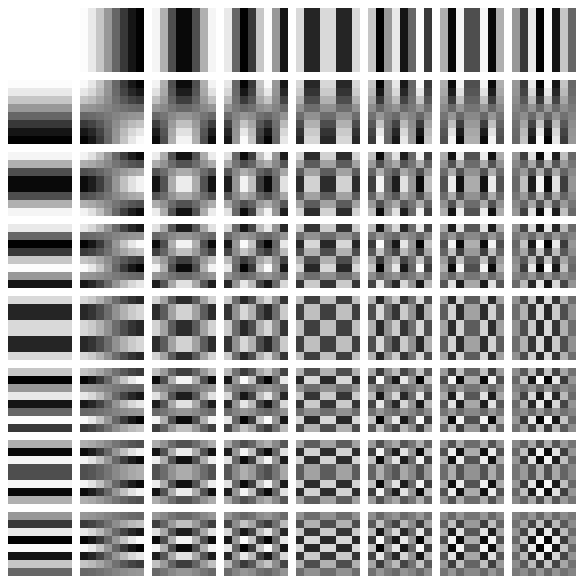
\includegraphics[width=0.6\textwidth]{../graphics/Dctjpeg_white.png}
    \caption[Short caption to special figure]{\textit{DCT patterns:} the values in the DCT coefficient matrix are weights for each of these patterns (known as \emph{basis functions}) which together construct the original 8$\times$8 image}
    \label{fig_dct}
\end{figure}



Every component in the frequency domain is now divided by a specific value. These values are given by the quantization matrix (which is different for different quality settings of the JPEG compression).

With $Q$ the quantization matrix, the quantized coefficient matrix $K$ is given by:

$$
K(k,n) = \textit{round} (\frac{G(k,n)}{Q(k,n)}) \textit{ for } k=0,1,2,...,7; n=0,1,2,...,7
$$

This rounding to the nearest integer is the only lossy part in the encoding, aside from possible downsampling of the $C_B$ and $C_R$ components.

\paragraph{Entropy encoding}
The values in this matrix are now losslessly compressed. The components are arranged in a ``zigzag'' order starting in the top left corner, which is favorable for run length encoding due to the zero values at the end. 


\paragraph{Decoding}
Decoding the image simply involves performing the opposite of all previous steps in reverse order. Of course, due to the rounding operation in the quantization step and the possible downsampling of chroma components the decoded image is likely different from the original. This difference may be visible to the human psychoperceptual system in the form of the artifacts described next.

\section{Artifacts}
Due to loss of information, visible artifacts are introduced to the image. Four main types of artifacts are generally observed under JPEG compression of images with a low quality setting. 

\paragraph{Ringing artifacts}
JPEG operates in the frequency domain, representing the image as a sum of oscillating waves. This is not suited for sharp edges, especially with low quality settings, these high frequency waves are rounded to zero. These artifacts are particulary visible in very high contrast images with sharp edges, such as text or simple vector images.

\paragraph{Block coding artifacts}
Due to the JPEG compression method working on 8$\times$8 blocks, discontinuities at the block boundaries may become visible. With a very low quality setting, only the DC coefficient may be available for every block, leading that block to be a single color. See figure \ref{fig:bc} for an example image where these artifacts are clearly visible.


\begin{figure}[ht]
    \centering
        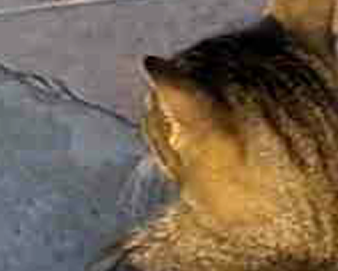
\includegraphics[width=0.6\textwidth]{../graphics/blocking.png}
    \caption[Short caption to special figure]{\textit{Block coding artifacts:} the 8$\times$8 blocks used internally are clearly visible}
    \label{fig:bc}
\end{figure}



\paragraph{Color distortion}
When the chroma components are subsampled, much of the fine detail is lost. The colors appear more washed out as they correspond to a larger area.

\paragraph{Posterization}
Posterization of an image is the loss of gradual change in tone. Whereas in the original image a color may smoothly go from one color to another, in the compressed image this may be a series of abrupt steps. This can be caused by both chroma component subsampling and quantization of these components. 


\section{Prior work}

Automated artifact removal methods exist that aim to remove or reduce these artifacts as a post-processing step. These range from hand-crafted algorithms to algorithms with learned parameters. \textit{TODO: Expand on non-DL approaches}

\subsection{Deep learning}

Every year the \emph{ImageNet Large Scale Visual Recognition Challenge (ILSVRC)}\footnote{http://image-net.org/} \cite{ILSVRC15} is held with as goal to create a system which can automatically determine the content of photographs. In 2010 and 2011 SVM approaches won the classification part of the competition, but ever since 2012 convolutional neural network (CNN) approaches - pioneered in this competition by Krizhevsky, Sutskever and Hinton - have won the competition \cite{alexnet}. These CNN approaches are the state of the art for automated image and speech recognition \cite{guodeep}\cite{abdelspeech}. Machine learning methods which use these connectionist models with many layers (making them \emph{deep}) is often referred to as \emph{deep learning}.

Contrary to regular methods such as SVMs (support vector machines), deep belief networks can automatically learn high level features in a supervised manner \cite{dlbook}. This is called representation learning. Features learned with automatic methods often outperform hand-crafted feature extractors. 

\bigskip

Deep learning methods work by learning and representing features in a hierarchical manner. For image classification for example, in the first layers simple shapes are used as features such as edges or corner. Deeper layers use (possibly non-linear) combinations of the features learned in earlier layers. If for instance a network is trained to recognize faces it may learn features such as eye color and nose shape in one layer, and learn that to best classify a certain person it is the combination of a high activation on the blue eye color, and a lower activation on the other colors.

\bigskip

This representation learning makes it a good candidate for the problem of JPEG compression artifact removal. With the advent of fully convolutional neural networks this can also be applied efficiently to dense prediction tasks like we are dealing with here\cite{long2015fully}. Such a network could learn to recognize the artifacts, and reconstruct the image before this artifact was introduced.

\subsection{Deep learning approaches for artifact removal}

\textit{TODO: Expand}

Dong et al. applied a deep learning model to the problem of artifact removal \cite{dong2015compression}. They proposed a four layer CNN, AR-CNN, which outperformed existing methods for artifact removal at the time of publication. They note that adding layers comes with great difficulty, as it may not converge. To counter this, they adopt a \emph{easy-to-hard} transfer strategy, where they first train a network to remove artifacts from images compressed with a high quality setting. Then they use the learned weights to initialize a network destined for lower quality setting JPEG images. The same strategy was also used to train deeper networks, where they initialized a five layer network with the weights of an earlier trained four layer network. Svoboda went deeper by adding layers with skip connections making it a residual architecture \cite{svoboda}. This likely makes it easier for the latent clean image to propagate through the network. Technically, however, not a residual function is learned, as opposed to the original ResNet architecture they concatenate the features instead of summing them.

Zhang et al. were able to improve upon these methods considerably \cite{zhang}. By instead of setting the original image as the training goal, the residual of this image was used as a target. This removes the necessity of a latent image representation in the hidden layers of the network. Also interesting is that this network was not only able to do JPEG artifact removal, but also Gaussian denoising and single image super-resolution.

\begin{table}[!t]
%% increase table row spacing, adjust to taste
\renewcommand{\arraystretch}{1.1}
% if using array.sty, it might be a good idea to tweak the value of
% \extrarowheight as needed to properly center the text within the cells
\caption{\emph{LIVE1 dataset validation metrics of prior methods for JPEG artifact removal. To do: Finish this, or leave it out.. Decisions..}}
\label{table_variables}
\centering
%% Some packages, such as MDW tools, offer better commands for making tables
%% than the plain LaTeX2e tabular which is used here.
\begin{tabular}{|lccc|}
\hline
\textsc{Method}&\textsc{PSNR}&\textsc{PSNR-B}&\textsc{SSIM}\\
\hline
\textbf{Quality factor 10}&&&\\
JPEG&27.77&0.7905&25.33\\
SA-DCT&28.65&0.8093&28.01\\
AR-CNN AR-CNN \cite{dong2015compression}&28.98&0.8217&28.70\\
L4 Residual \cite{svoboda}&29.08&0.824&28.71\\
CAS-CNN MS loss \cite{CavigelliHB16}&29.36&0.830&28.92\\
CAS-CNN w/ loss FT \cite{CavigelliHB16}&29.44&0.833&29.19\\
&&&\\
\textbf{Quality factor 20}&&&\\
JPEG&30.07&0.8683&27.57\\
SA-DCT&30.81&0.8781&29.82\\
AR-CNN \cite{dong2015compression}&31.29&0.8871&30.76\\
L4 Residual \cite{svoboda}&31.42&0.890&30.83\\
L8 Residual \cite{svoboda}&31.51&0.891&30.92\\
CAS-CNN MS loss \cite{CavigelliHB16}&31.67&0.894&30.84\\
CAS-CNN w/ loss FT \cite{CavigelliHB16}&31.70&0.895&30.88\\
&&&\\

%\textbf{BSDS500 Dataset QF10}&&&\\
%JPEG&26.62&0.7904&23.54\\
%AR-CNN&27.71&0.8192&27.04\\
%L4 Residual&28.75&0.800&28.29\\

&&&\\


\hline

\end{tabular}
\end{table}


\subsection{Sparse coding approaches}
\textit{TODO}

\section{Exploiting JPEG redundancies further with color}
Most, if not all, prior work on JPEG compression only consider grayscale images. As the Y, Cb and Cr components of the image are processed in the same way it is argued that these methods also apply color images by simply applying it to each of these components independently. While it is true that this works, the components are not processed in exactly the same way. First of all, for the chroma components often a quantization matrix with higher values is used (which means it is more lossy). Secondly, it is very common that the chroma components are first downscaled (e.g. with a 2x2 factor) prior to splitting into the 8$\times$8 pixel blocks. To apply methods only trained on grayscale images, one should thus first downscale the color components to match the 8x8 DCT blocks. 

JPEG compression artifact reduction mostly relies on the redundancies of adjacent 8$\times$8 blocks of pixels, especially those that operate (partially) in the DCT domain. The DCT blocks of the chroma components, however, describe a 16$\times$16 block in the original image. These redundancies are thus at a larger spatial scale than the Y component's block redundancies. As the luma and chrominance are likely very highly correlated on a spatially local scale, the larger scale information of the chroma channels can be used to improve the luma channel, and vice versa.

Also, due to the more aggressive quantization of the chroma channels, the possible interval of original value of one of the DCT coefficients is large, especially for the high frequency components. This is finer for the luma channel, this information can be used to better infer the original coefficients.




\section{Evaluative measures}
To determine the efficacy of a method for compression artifact removal several quantitative methods are available. Generally it is a distance measure between the restored image and the original image prior to compression.

\paragraph{Mean squared error (MSE)}
MSE is the simplest measure, often used as the loss function for methods that rely on optimization. It is simply the square of the distance per pixel averaged over all pixels in the dataset. It is given by

$$
\textit{MSE}= \frac{1}{\sqrt{N}} \sum^N_{i=1}({x}_i - y_i)^2,
$$
with $N$ the total amount of pixels, $y$ a predicted pixel, and ${x}$ the pixel prior to compression.

\paragraph{Peak signal-to-noise ratio (PSNR)}
Peak signal-to-noise ratio is given by the the ratio of noise to the maximum possible power of the signal, which in this case is the image. It is most often expressed on the logarithmic decibel scale. PSNR in dB is given by
$$
\textit{PSNR} = 10 \cdot \textit{log}_{10}(\frac{\textit{DEPTH}^2}{\textit{MSE}}),
$$
with $\textit{DEPTH}$ the maximum pixel value of the image (255 for 8 bit images). 

\paragraph{Structural similarity (SSIM)}
The Structural Similarity index was developed as an improvement to MSE and PSNR with the goal of being more consistent with how humans perceive images\cite{wang2004imagessim}. The index consists of a weighed combination of comparison measures between samples of luminance, constrast and structure across the whole image. These samples are taken with a sliding window approach (generally with an 8$\times$8 window).

\paragraph{Peak signal-to-noise ratio including blocking effects (PSNR-B)}
PSNR-B is an adaptation of the PSNR introduced by Yim et al. to account for the blocking effect often introduced by image or movie compression algorithms \cite{yim2011qualitypsnrb}. They introduce the mean squared error including blocking effects \textit{MSE-B}, which includes a blocking effect factor \textit{BEF} which is determined from the pixel values on the boundary of the blocks (8$\times$8 in the JPEG case):

$$
\textit{MSE-B} = \textit{MSE} + \textit{BEF},
$$

the PSNR-B then becomes

$$
\textit{PSNR-B} = 10 \cdot \textit{log}_{10}(\frac{\textit{DEPTH}^2}{\textit{MSE-B}}).
$$

%%%
\section{Datasets}
A large amount of different datasets exist for benchmarking and training of image processing, segmentation and classification techniques. For the compression artifact reduction task any image is potentially suitable as ground truth. Ideally, however, the image used as ground truth (prior to JPEG compression) is uncompressed or compressed with a lossless compression algorithm. Below is a list of datasets used in prior work, and other datasets identified as usable in this context. The majority of these datasets are images that have been compressed with a lossy algorithm, albeit it with a high quality factor. \textit{TODO: some accompanying text on each of these.}

\paragraph{LIVE1 dataset \cite{liveDatabase}} 29 grayscale images.

\paragraph{Berkeley Segmentation Dataset (BSD500) \cite{bsd500}} Training set of 200 images, validation set of 100 images and a test set of 100 images. 

\paragraph{Places365-Standard dataset \cite{places2}} Training set of 1,803,460 images, validation set of 36,500 images and test set of 328,500 images.

\paragraph{Uncompressed Colour Image Dataset (UCID) \cite{ucid}} 1338 truly uncompressed images taken with the same camera.

\section{Relevance and impact}{}

To save on bandwidth and storage costs, images are often compressed using a lossy compression algorithm. The compression ratios of these lossy methods is often much better than those of lossless compression algorithms. This compression may result in a noticable degradation in image quality.

This compression often happens unknowningly for the average user. An image attached to a Twitter tweet, uploaded to other social media, or saved in a cloud storage service (such as Dropbox) may be compressed without the user knowing. Also, sometimes digital cameras do not even support the option of storing a lossless version of the original image. 

Removing the artifacts introduced by lossy compression can allow for restoring the higher quality original image in these cases.